\section{High-Level Language-Based Programming}


\subsection{Python}


\par
There has been a lot of progress in GPU programming using Python and the ecosystem is still evolving.
There are a couple of options available to work with GPU.


\subsubsection{CuPy}


\par
CuPy~\cite{cupy} is a NumPy/SciPy-compatible data array library used on GPU.
It has been developed for NVIDIA GPUs but as experimental support for AMD GPUs.
CuPy has a highly compatible interface with NumPy and SciPy.
As stated on its official website,~\textit{\lq\lq All you need to do is just replace numpy and scipy with cupy and cupyx.scipy in your Python code\rq\rq}.
If you know NumPy, CuPy is a very easy way to get started on the GPU.


\subsubsection{cuDF}


\par
RAPIDS~\cite{rapids} is a high level packages collections which implement CUDA functionalities and API with Python bindings.
It only supports NVIDIA GPUs.
cuDF~\cite{cudf} belongs to RAPIDS and is the library for manipulating data frames on GPU.
cuDF provides a pandas-like API, so if you are familiar with Pandas~\cite{pandas}, you can accelerate your work without knowing too much CUDA programming.


\subsubsection{PyCUDA}


\par
PyCUDA~\cite{pycuda} is a Python programming environment for CUDA.
It allows users to access to NVIDIA’s CUDA API from Python.
PyCUDA is powerful library but only runs on NVIDIA GPUs.
Knowledge of CUDA programming is needed.


\subsubsection{Numba}


\par
Numba~\cite{numba} allows users to JIT~\cite{jit} compile Python code to run fast on CPUs, but can also be used for JIT compiling for GPUs.
In the following we will focus on using Numba, which supports GPUs from both NVIDIA and AMD.
It should be noted that Numba supported AMD GPUs up until version 0.53 but has since deprecated the support.


\par
Numba supports GPU programming by directly compiling a restricted subset of Python code into kernels and device functions following the execution model.
Kernels written in Numba appear to have direct access to NumPy arrays.
NumPy arrays are transferred between the CPU and the GPU automatically.


\par
Using~\textbf{ufuncs} (and generalized ufuncs (\textbf{gufunc})) is the easiest way to run on a GPU with Numba, and it requires minimal understanding of GPU programming.
Numba~\textbf{\textcolor{red}{@vectorize}} will produce a ufunc-like object.
This object is a close analog but not fully compatible with a regular NumPy ufunc.
Generating a ufunc for GPU requires the explicit type signature and target attribute.


\paragraph{Numba ufunc.}
Here are multiple samples for a simple mathematical problem using Numba~\textbf{ufunc} for CPU (List~\ref{lst:06_python_numba_ufunc_cpu}) and GPU (List~\ref{lst:06_python_numba_ufunc_gpu}), as well as a reference sample without using Numba~\textbf{ufunc} (List~\ref{lst:06_python_numba_ufunc}).


\lstinputlisting[language=python, firstline=16, lastline=21, caption={A simple mathematical problem using Numba~\textbf{ufunc} for CPU in Python.}, label={lst:06_python_numba_ufunc_cpu}, xleftmargin=0.05\textwidth, xrightmargin=0.05\textwidth]{code_examples/06_python_numba_ufunc.py}


\lstinputlisting[language=python, firstline=30, lastline=35, caption={A simple mathematical problem using Numba~\textbf{ufunc} for GPU in Python.}, label={lst:06_python_numba_ufunc_gpu}, xleftmargin=0.05\textwidth, xrightmargin=0.05\textwidth]{code_examples/06_python_numba_ufunc.py}


\lstinputlisting[language=python, firstline=4, lastline=7, caption={A simple mathematical problem in Python.}, label={lst:06_python_numba_ufunc}, xleftmargin=0.05\textwidth, xrightmargin=0.05\textwidth]{code_examples/06_python_numba_ufunc.py}


\par
The benchmark computational results for the simple mathematical problem using Numba~\textbf{ufunc} for CPU and GPU are provided in List~\ref{lst:06_python_numba_ufunc_cpu_benchmark} and List~\ref{lst:06_python_numba_ufunc_gpu_benchmark}, respectively, as well as for the reference sample without using Numba~\textbf{ufunc} in List~\ref{lst:06_python_numba_ufunc_benchmark}.


\lstinputlisting[language=python, firstline=20, lastline=27, caption={The benchmark computational result for the simple mathematical problem using Numba~\textbf{ufunc} for CPU in Python.}, label={lst:06_python_numba_ufunc_cpu_benchmark}, xleftmargin=0.05\textwidth, xrightmargin=0.05\textwidth]{code_examples/06_python_numba_ufunc_benchmark.py}


\lstinputlisting[language=python, firstline=36, lastline=43, caption={The benchmark computational result for the simple mathematical problem using Numba~\textbf{ufunc} for GPU in Python.}, label={lst:06_python_numba_ufunc_gpu_benchmark}, xleftmargin=0.05\textwidth, xrightmargin=0.05\textwidth]{code_examples/06_python_numba_ufunc_benchmark.py}


\lstinputlisting[language=python, firstline=4, lastline=11, caption={The benchmark computational result for the simple mathematical problem in Python.}, label={lst:06_python_numba_ufunc_benchmark}, xleftmargin=0.05\textwidth, xrightmargin=0.05\textwidth]{code_examples/06_python_numba_ufunc_benchmark.py}


\par
It should be noted that the Numba~\textbf{\textcolor{red}{@vectorize}} is limited to scalar arguments in the core function, for multi-dimensional arrays arguments, the~\textbf{\textcolor{red}{@guvectorize}} is used.
In addition, one should never implement things like matrix multiplication by oneself since there are plenty of highly optimized libraries available!.


\paragraph{Numba gufunc.}
Consider the following examples for the matrix multiplication using Numba~\textbf{gufunc} for CPU (List~\ref{lst:06_python_numba_gufunc_cpu}) and GPU (List~\ref{lst:06_python_numba_gufunc_gpu}), as well as a reference sample without using Numba~\textbf{gufunc} (List~\ref{lst:06_python_numba_gufunc}).


\lstinputlisting[language=python, firstline=21, lastline=32, caption={A simple mathematical problem using Numba~\textbf{gufunc} for CPU in Python.}, label={lst:06_python_numba_gufunc_cpu}, xleftmargin=0.05\textwidth, xrightmargin=0.05\textwidth]{code_examples/06_python_numba_gufunc.py}


\lstinputlisting[language=python, firstline=41, lastline=52, caption={A simple mathematical problem using Numba~\textbf{gufunc} for GPU in Python.}, label={lst:06_python_numba_gufunc_gpu}, xleftmargin=0.05\textwidth, xrightmargin=0.05\textwidth]{code_examples/06_python_numba_gufunc.py}


\lstinputlisting[language=python, firstline=4, lastline=12, caption={A simple mathematical problem in Python.}, label={lst:06_python_numba_gufunc}, xleftmargin=0.05\textwidth, xrightmargin=0.05\textwidth]{code_examples/06_python_numba_gufunc.py}


\par
The benchmark computational results for the matrix multiplication using Numba~\textbf{gufunc} for CPU and GPU are provided in List~\ref{lst:06_python_numba_gufunc_cpu_benchmark} and List~\ref{lst:06_python_numba_gufunc_gpu_benchmark}, respectively.


\lstinputlisting[language=python, firstline=4, lastline=10, caption={The benchmark computational result for the matrix multiplication using Numba~\textbf{gufunc} for CPU in Python.}, label={lst:06_python_numba_gufunc_cpu_benchmark}, xleftmargin=0.05\textwidth, xrightmargin=0.05\textwidth]{code_examples/06_python_numba_gufunc_benchmark.py}


\lstinputlisting[language=python, firstline=19, lastline=25, caption={The benchmark computational result for the matrix multiplication using Numba~\textbf{gufunc} for GPU in Python.}, label={lst:06_python_numba_gufunc_gpu_benchmark}, xleftmargin=0.05\textwidth, xrightmargin=0.05\textwidth]{code_examples/06_python_numba_gufunc_benchmark.py}


\par
From the examples listed above, it is clear that the Numba automatically did a lot of things for us:
\begin{itemize}
    \item Memory was allocated on GPU
    \item Data was copied from CPU and GPU
    \item The kernel was configured and launched
    \item Data was copied back from GPU to CPU
\end{itemize}


\par
Therefore, using Numba~\textbf{ufunc} (\textbf{gufunc}) for GPU processing is straightforward, but this approach may not always yield optimal performance due to automatic handling of data transfer to and from the GPU, as well as kernel launching.
Additionally, in practice, not every function can be constructed as a~\textbf{ufunc} (\textbf{gufunc}).

\par
To gain greater control and flexibility, one may need to craft their own kernels and manually manage data transfer.
Refer to the~\href{https://enccs.github.io/hpda-python/parallel-computing/}{Python for HPDA} resource for guidance on implementing such techniques using Numba.


% -------------------------------------------------------------------- %


\subsection{Julia}


\par
Julia~\cite{julia} has the first-class support for GPU programming through the following packages that target GPUs from all three major vendors:
\begin{itemize}
    \item~\textbf{\textcolor{brown}{CUDA.jl}} for NVIDIA GPUs~\cite{cudajl}
    \item~\textbf{\textcolor{brown}{AMDGPU.jl}} for AMD GPUs~\cite{amdgpujl}
    \item~\textbf{\textcolor{brown}{oneAPI.jl}} for Intel GPUs~\cite{oneapijl}
    \item~\textbf{\textcolor{brown}{Metal.jl}} for Apple M-series GPUs~\cite{metaljl}
\end{itemize}


\par
\textbf{\textcolor{brown}{CUDA.jl}} is the most mature,~\textbf{\textcolor{brown}}{AMDGPU.jl} is somewhat behind but still ready for general use, while~\textbf{\textcolor{brown}{oneAPI.jl}} and~\textbf{\textcolor{brown}{Metal.jl}} are functional but might contain bugs, miss some features and provide sub-optimal performance.
Their respective APIs are however completely analogous and translation between libraries is straightforward.
The libraries offer both user-friendly~\textbf{high-level abstractions} (the array interface and higher-level abstractions) that require little programming effort, and a~\textbf{low-level approach} for writing kernels for fine-grained control.


\par
Installing these packages is done with the Julia package manager shown in List~\ref{lst:06_julia_gpu_package}.


\lstinputlisting[language=python, firstline=1, lastline=22, caption={Installing relevant packages for different GPUs using the Julia package manager.}, label={lst:06_julia_gpu_package}, xleftmargin=0.05\textwidth, xrightmargin=0.05\textwidth]{code_examples/06_julia_gpu_package.jl}


\par
To use the Julia GPU stack, one needs to have the relevant GPU drivers and programming toolkits installed.
GPU drivers are already installed on HPC systems while on your own machine you will need to install them yourself (see $e.g.$ instructions from NVIDIA~\cite{nvidia_driver}).
Programming toolkits for CUDA can be installed automatically through Julia’s artifact system upon the first usage:
\lstinputlisting[language=python, firstline=31, lastline=32, xleftmargin=0.05\textwidth, xrightmargin=0.05\textwidth]{code_examples/06_julia_gpu_package.jl}


\subsubsection{Array interface}


\par
GPU programming with Julia can be as simple as using a different array type instead of regular~\textbf{\textcolor{red}{Base.Array}} arrays:
\begin{itemize}
    \item~\textbf{\textcolor{red}{CuArray}} from CUDA.jl for NVIDIA GPUs
    \item~\textbf{\textcolor{red}{ROCArray}} from AMDGPU.jl for AMD GPUs
    \item~\textbf{\textcolor{red}{oneArray}} from oneAPI.jl for Intel GPUs
    \item~\textbf{\textcolor{red}{MtlArray}} from Metal.jl for Apple GPUs
\end{itemize}


\par
These array types closely resemble~\textcolor{red}{\textbf{Base.Array}} which enables us to write generic code which works on both types.
The code in List~\ref{lst:06_julia_copy_array} copies an array to the GPU and executes a simple operation on the GPU.


\lstinputlisting[language=python, firstline=1, lastline=34, caption={Copying an array to GPU and then executing a simple operation on GPU.}, label={lst:06_julia_copy_array}, xleftmargin=0.05\textwidth, xrightmargin=0.05\textwidth]{code_examples/06_julia_copy_array.jl}


\par
Moving an array back from the GPU to the CPU is simple using the command:
\lstinputlisting[language=python, firstline=40, lastline=40, xleftmargin=0.05\textwidth, xrightmargin=0.05\textwidth]{code_examples/06_julia_copy_array.jl}


\par
Let’s have a look at a more realistic example: matrix multiplication.
We create two random arrays, one on the CPU and one on the GPU, and compare the performance using the~\textbf{BenchmarkTools} package~\cite{benchmarktools}.
The code examples running on different GPUs are shown in List~\ref{lst:06_julia_benckmarktool}.


\lstinputlisting[language=python, caption={Code examples for the matrix multiplication executed on different GPUs.}, label={lst:06_julia_benckmarktool}, xleftmargin=0.05\textwidth, xrightmargin=0.05\textwidth]{code_examples/06_julia_benckmarktool.jl}


\subsubsection{Vendor libraries}


\par
Support for using GPU vendor libraries from Julia is currently most mature on NVIDIA GPUs.
NVIDIA libraries contain pre-compiled kernels for common operations like matrix multiplication (cuBLAS), fast Fourier transforms (cuFFT), linear solvers (cuSOLVER), $etc$.
These kernels are wrapped in~\textbf{\textcolor{brown}{CUDA.jl}} and can be used directly with~\textbf{\textcolor{red}{CuArray}}, as shown in List~\ref{lst:06_julia_library}.


\lstinputlisting[language=python, caption={Code examples using precompiled kernels wrapped in~\textbf{\textcolor{brown}{CUDA.jl}} for NVIDIA GPU.}, label={lst:06_julia_library}, xleftmargin=0.05\textwidth, xrightmargin=0.05\textwidth]{code_examples/06_julia_library.jl}


\par
For~\textbf{\textcolor{brown}{AMDGPU.jl}}, it currently supports some of the ROCm libraries:
\begin{itemize}
    \item rocBLAS for BLAS support
    \item rocFFT for FFT support
    \item rocRAND for RNG support
    \item MIOpen for DNN support
\end{itemize}


\subsubsection{Higher-order abstractions}


\par
A powerful way to program GPUs with arrays is through Julia’s higher-order array abstractions.
The simple element-wise addition we saw above, $a$~$.+=$~1, is an example of this, but more general constructs can be created with~\textbf{\textcolor{red}{broadcast}},~\textbf{\textcolor{red}{map}},~\textbf{\textcolor{red}{reduce}}, and~\textbf{\textcolor{red}{accumulate}}, as shown in List~\ref{lst:06_julia_high_order_abstraction}.


\lstinputlisting[language=python, caption={Abstractions used to create constructs for element-wise addition.}, label={lst:06_julia_high_order_abstraction}, xleftmargin=0.05\textwidth, xrightmargin=0.05\textwidth]{code_examples/06_julia_high_order_abstraction.jl}


\subsubsection{Writing kernels}


\par
Not all algorithms can be made to work with the higher-level abstractions in~\textbf{\textcolor{brown}{CUDA.jl}}.
In such cases it’s necessary to explicitly write our own GPU kernels.


\par
Similar to writing kernels in CUDA or HIP, we use a special function to return the index of the GPU thread which executes it ($e.g.$, $threadIdx().x$ for NVIDIA and $workitemIdx().x$ for AMD), and two additional functions to parallelise over multiple blocks ($e.g.$, $blockDim().x()$ and $blockIdx().x()$ for NVIDIA, and $workgroupDim().x()$ and $workgroupIdx().x()$ for AMD), as shown in Fig.~\ref{fig:mapping_blocks_2_SMs}.


\begin{figure}[!h]
\centering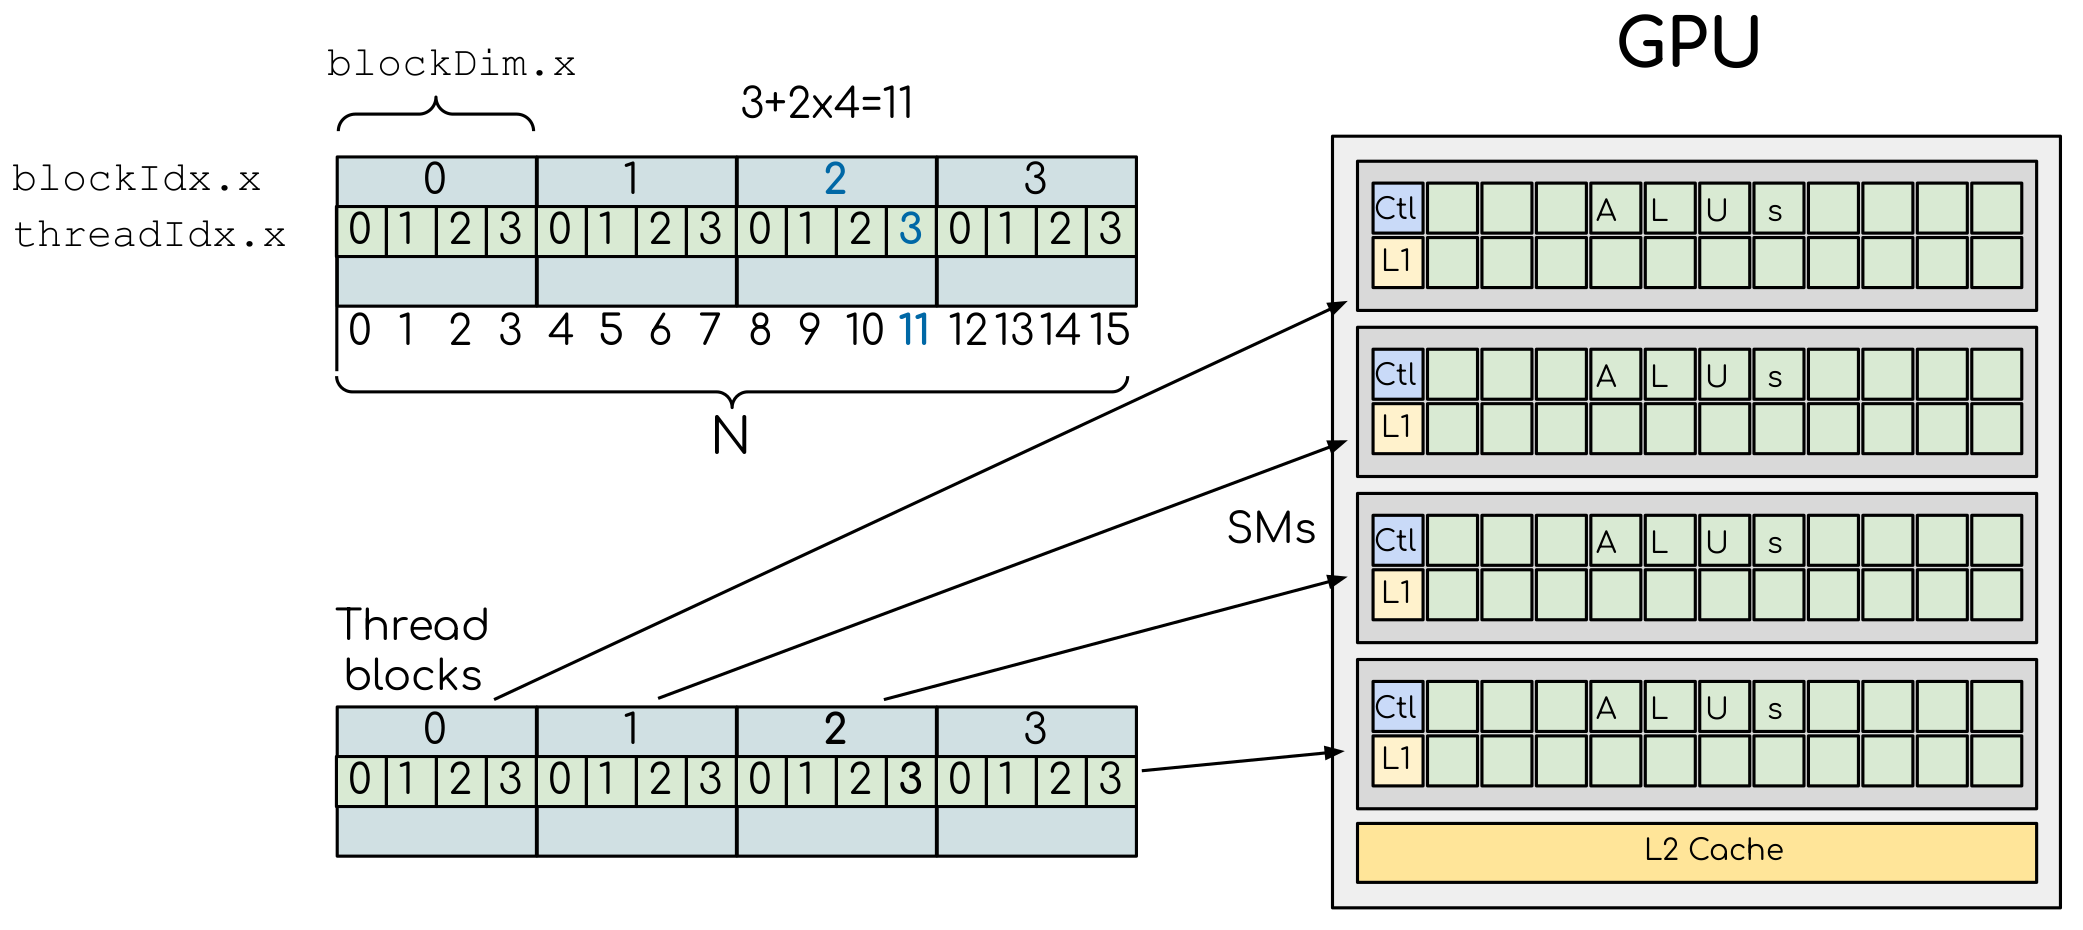
\includegraphics[width=0.8\textwidth]{fig_hardware/mapping_blocks_2_SMs.png}
\caption{Mapping thread and thread block indexes to SMPs on GPU.}\label{fig:mapping_blocks_2_SMs}
\end{figure}


\par
Below is list of code examples of vector addition kernel for NVIDIA, AMD, Intel and Apple GPUs in the subdirectory of this repository~\cite{gpu-programming-examples}.

\textbf{\textcolor{brown}{content/examples/code_examples/06_julia_own_kernel_nvidia.jl}}

\textbf{\textcolor{brown}{content/examples/code_examples/06_julia_own_kernel_amd.jl}}

\textbf{\textcolor{brown}{content/examples/code_examples/06_julia_own_kernel_intel.jl}}

\textbf{\textcolor{brown}{content/examples/code_examples/06_julia_own_kernel_apple.jl}}



\par
Two additional points should be address here.
\begin{itemize}
    \item \textbf{Restrictions in kernel programming}: Within kernels, most of the Julia language is supported with the exception of functionality that requires the Julia runtime library. This means one cannot allocate memory or perform dynamic function calls, both of which are easy to do accidentally!
    \item \textbf{1D, 2D and 3D}:~\textbf{\textcolor{brown}{CUDA.jl}} and~\textbf{\textcolor{brown}{AMDGPU.jl}} support indexing in up to 3 dimensions ($x$, $y$ and $z$, $e.g.$, $threadIdx().x$ and $workitemIdx().x$). This is convenient for multidimensional data where thread blocks can be organised into 1D, 2D or 3D arrays of threads.
\end{itemize}


\par
More reading materials related to the topics discussed above are available at:
\begin{itemize}
    \item~\href{https://enccs.github.io/hpda-python/parallel-computing/}{Python for HPDA} (ENCCS)
    \item~\href{https://uppmax.github.io/HPC-python/}{Python in HPC} (UPPMAX-HPC2N)
    \item~\href{https://enccs.github.io/julia-for-hpc/}{Julia for HPC}
\end{itemize}

